\element{PFSStrat}{
\begin{question}{pfsstrat 01a}
Soit le modèle suivant. On cherche, en statique, la relation entre le couple moteur, la pesanteur et le ressort. 
On cherche à savoir quelle pièce, ou quel ensemble de pièces commencer par isoler. 
\begin{center}
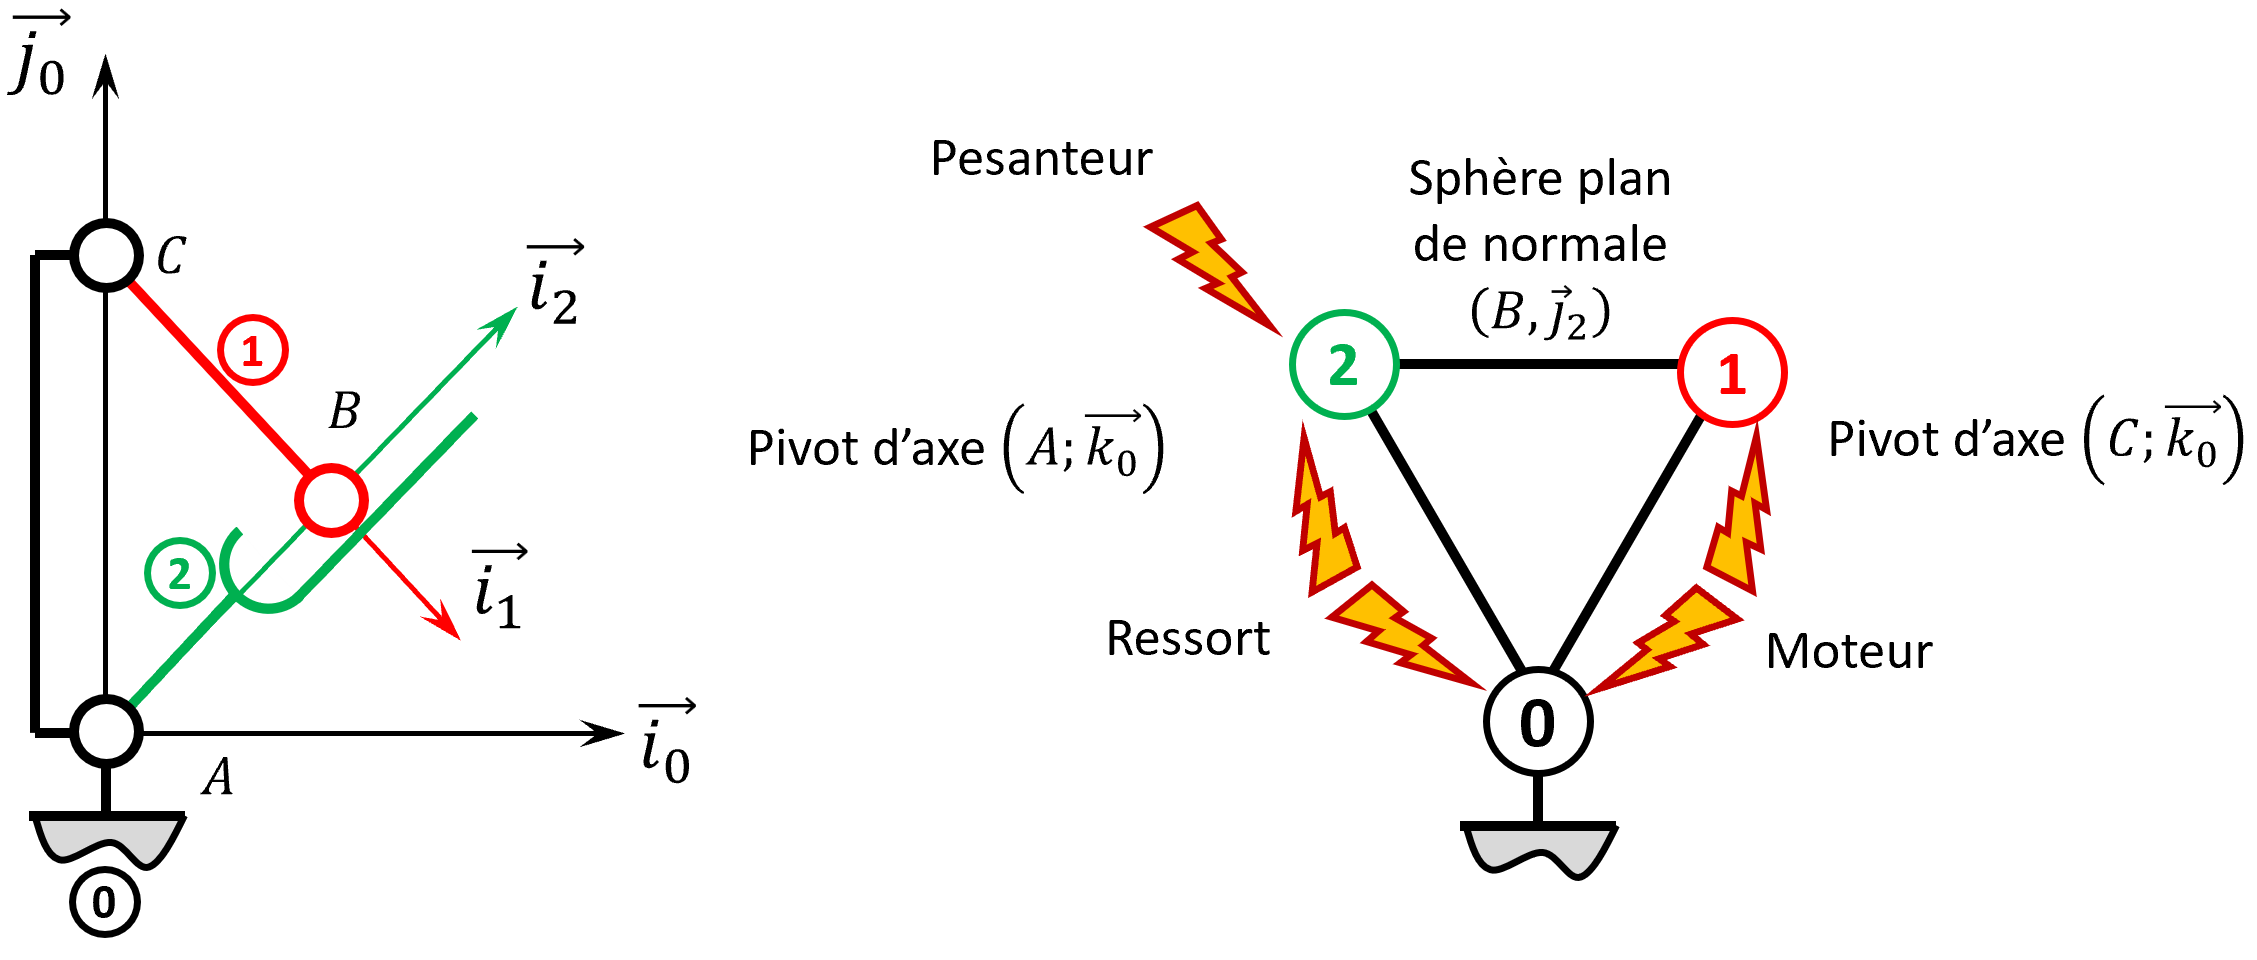
\includegraphics[width=.95\linewidth]{pfs_strategie_sympact_01}
\end{center}
	\begin{reponses}	
	\bonne Peu importe.
	\mauvaise On commence par isoler 1. 
	\mauvaise On commence par isoler 2.
	\mauvaise On commence par isoler 1+2.
	\end{reponses}
\end{question}\\}

\element{PFSStrat}{
\begin{question}{pfsstrat 02a}
Soit le modèle suivant. On cherche, en statique, la relation entre le couple moteur, la pesanteur et le ressort. 
On a isolé 1. Quelle équation est-il intéressante d'écrire ?
\begin{center}
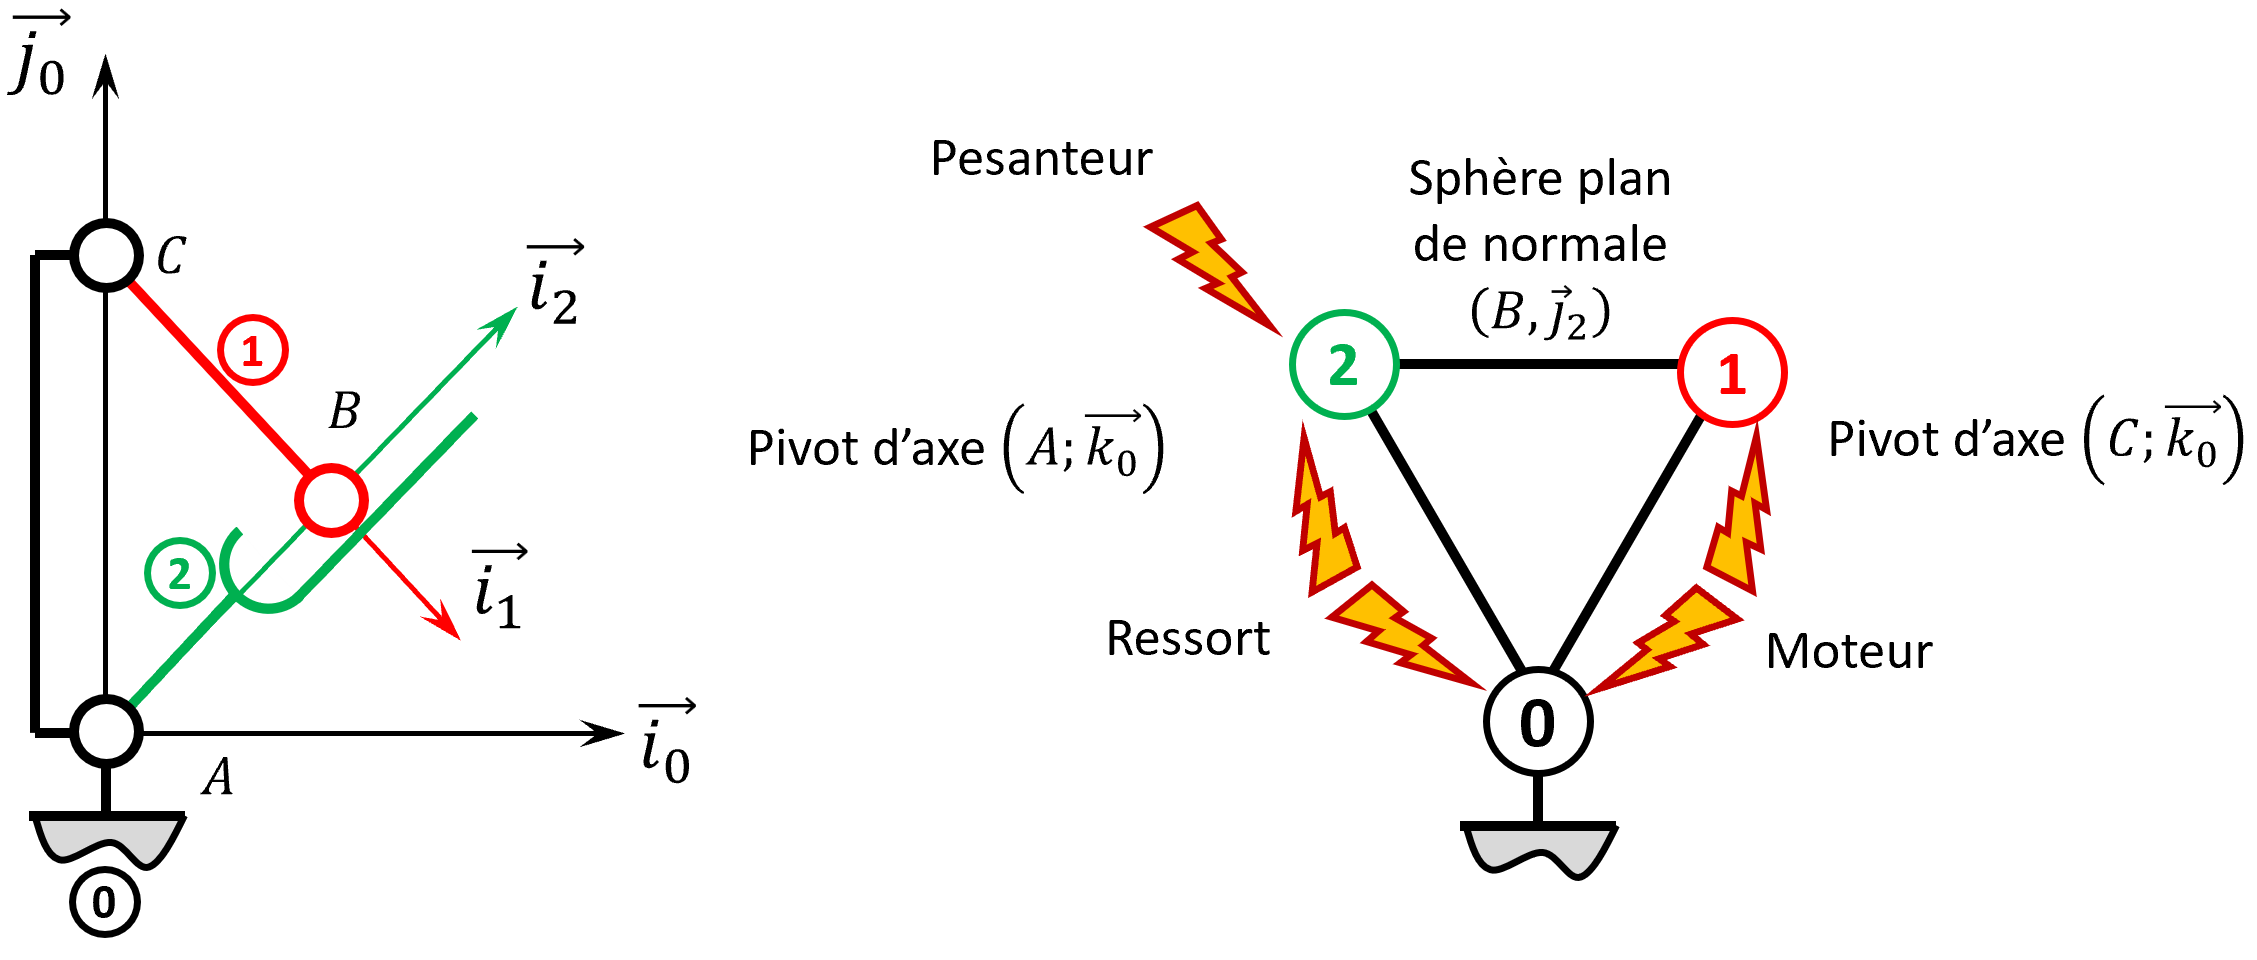
\includegraphics[width=.95\linewidth]{pfs_strategie_sympact_01}
\end{center}
	\begin{reponses}	
	\bonne le TMS.
	\mauvaise le TRS.
	\mauvaise en $A$.
	\mauvaise en $B$.
	\bonne en $C$.
	\mauvaise en projection sur $\vi{0}$.
	\mauvaise en projection sur $\vj{0}$.		
	\mauvaise en projection sur $\vi{1}$.
	\mauvaise en projection sur $\vj{1}$.		
	\mauvaise en projection sur $\vi{2}$.
	\mauvaise en projection sur $\vj{2}$.		
	\bonne en projection sur $\vz{0}$.		
	\end{reponses}
\end{question}\\}

\element{PFSStrat}{
\begin{question}{pfsstrat 02b}
Soit le modèle suivant. On cherche, en statique, la relation entre le couple moteur, la pesanteur et le ressort. 
On a isolé 2. Quelle équation est-il intéressante d'écrire ?
\begin{center}
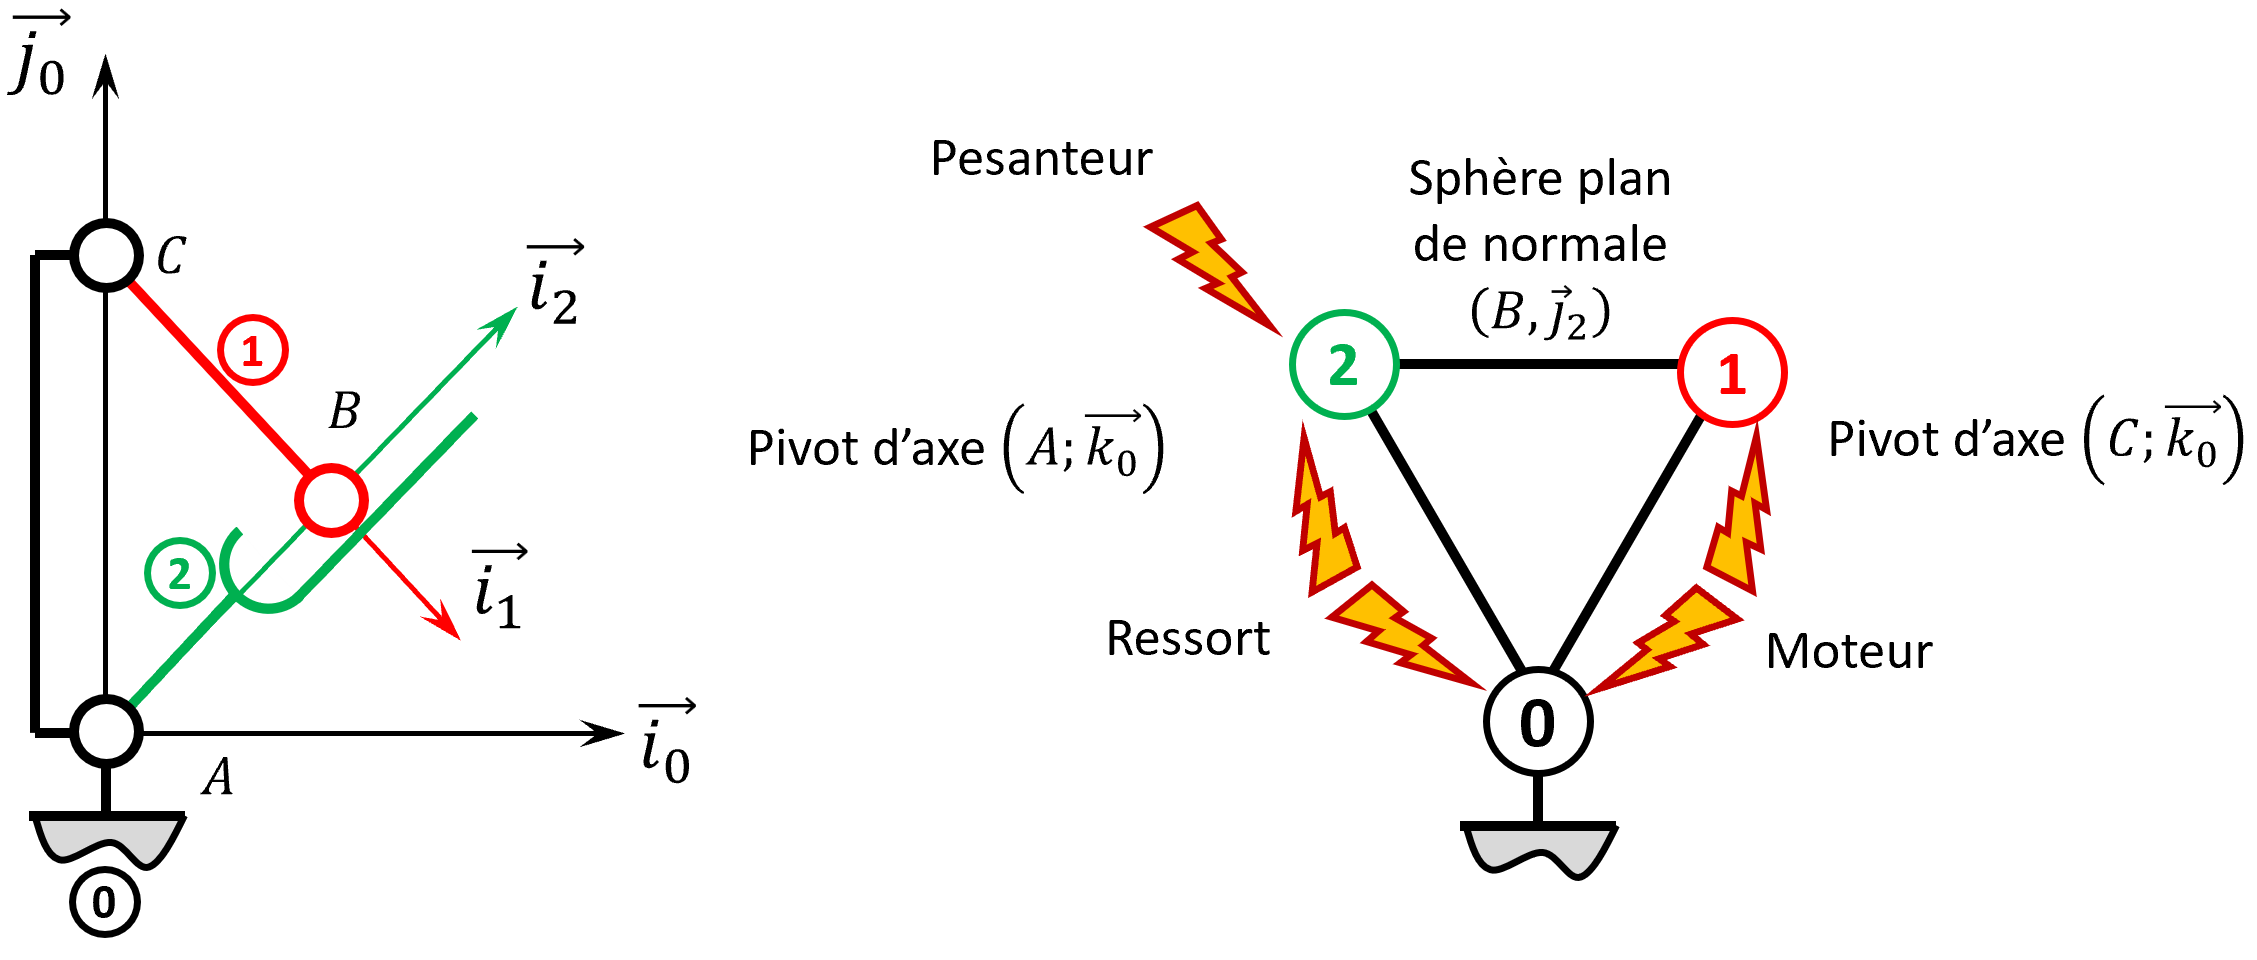
\includegraphics[width=.95\linewidth]{pfs_strategie_sympact_01}
\end{center}
	\begin{reponses}	
	\bonne le TMS.
	\mauvaise le TRS.
	\bonne en $A$.
	\mauvaise en $B$.
	\mauvaise en $C$.
	\mauvaise en projection sur $\vi{0}$.
	\mauvaise en projection sur $\vj{0}$.		
	\mauvaise en projection sur $\vi{1}$.
	\mauvaise en projection sur $\vj{1}$.		
	\mauvaise en projection sur $\vi{2}$.
	\mauvaise en projection sur $\vj{2}$.		
	\bonne en projection sur $\vz{0}$.		
	\end{reponses}
\end{question}\\}